\documentclass[11pt,a4paper]{article}

% --- PACKAGES ---
\usepackage[utf8]{inputenc}
\usepackage[T1]{fontenc}
\usepackage{lmodern}
\usepackage[margin=1in,headheight=14pt]{geometry}
\usepackage{graphicx}
\usepackage{float}
\usepackage{booktabs}
\usepackage{array}
\usepackage{enumitem}
\usepackage{listings}
\usepackage{xcolor}
\usepackage{fancyhdr}
\usepackage{hyperref}
\usepackage{titlesec}
\usepackage{tabularx}

% --- PALETTE ---
\definecolor{ink}{RGB}{27, 67, 72}
\definecolor{teal}{RGB}{32, 120, 128}
\definecolor{clay}{RGB}{186, 101, 58}
\definecolor{body}{RGB}{40, 44, 48}
\definecolor{softbg}{RGB}{244, 248, 247}
\definecolor{edge}{RGB}{214, 222, 220}
\definecolor{codebg}{RGB}{247, 248, 246}
\definecolor{kw}{RGB}{27, 67, 120}
\definecolor{str}{RGB}{150, 40, 40}
\definecolor{cmt}{RGB}{30, 120, 60}

% --- HEADINGS ---
\titleformat{\section}{\normalfont\Large\bfseries\color{ink}}{\thesection}{1em}{}[\textcolor{clay}{\titlerule}]
\titleformat{\subsection}{\normalfont\large\bfseries\color{teal}}{\thesubsection}{1em}{}

% --- LISTS ---
\setlist{topsep=3pt, itemsep=2pt, parsep=0pt}

% --- LISTINGS ---
\lstset{
  language=Python,
  backgroundcolor=\color{codebg},
  basicstyle=\ttfamily\footnotesize\color{body},
  keywordstyle=\bfseries\color{kw},
  stringstyle=\color{str},
  commentstyle=\itshape\color{cmt},
  numbers=left,
  numberstyle=\tiny\color{gray},
  numbersep=6pt,
  showstringspaces=false,
  breaklines=true,
  frame=single,
  rulecolor=\color{edge},
  tabsize=4,
  captionpos=b
}
\lstdefinestyle{shell}{language=bash, numbers=none}

% --- PATHS / HEADERS ---
\graphicspath{{img/}}
\pagestyle{fancy}
\fancyhf{}
\fancyhead[L]{\small\color{gray}LensMetrics --- Evaluated Project Report}
\fancyhead[R]{\small\color{gray}Computer Vision}
\fancyfoot[L]{\small\color{gray}Trisha (24BAC10012)}
\fancyfoot[R]{\small\color{gray}Page \thepage}
\renewcommand{\headrulewidth}{0.4pt}
\renewcommand{\footrulewidth}{0.4pt}

\hypersetup{
  colorlinks=true, linkcolor=ink, urlcolor=teal,
  pdftitle={LensMetrics - Smart Photo Quality and Structure Inspector},
  pdfauthor={Trisha (24BAC10012)},
  pdfsubject={Computer Vision Evaluated Project},
  pdfkeywords={Python, OpenCV, photo quality, face detection, edge detection, pytest}
}

\begin{document}

% ================= COVER =================
\begin{titlepage}
  \centering
  \vspace*{1.2cm}
  {\Huge\bfseries\color{ink} LENSMETRICS \par}
  \vspace{0.5cm}
  {\Large\color{teal} Smart Photo Quality \& Structure Inspector \par}
  \vspace{0.4cm}
  \textcolor{clay}{\rule{0.55\textwidth}{2pt}}
  \vspace{1.8cm}

  {\Large\bfseries Computer Vision (CSE3010) \par}
  \vspace{0.2cm}
  {\large Evaluated Course Project \par}
  \vspace{2.8cm}

  {\large
  \textbf{Submitted By:} \\[0.3em]
  {\Large\textsc{Trisha}} \\[0.2em]
  \textbf{Registration Number:} 24BAC10012 \\[0.5em]
  \textbf{Stack:} Python, OpenCV, NumPy \\[0.2em]
  \textbf{Testing:} Pytest \par}

  \vfill
  {\large Academic Year: 2026--27 \par}
  \vspace*{1cm}
\end{titlepage}

% ================= CONTENTS =================
\newpage
\pagenumbering{roman}
\tableofcontents
\newpage
\pagenumbering{arabic}

% ================= 1 =================
\section{Overview}
Everyday photo folders grow faster than anyone curates them. Some shots are
soft, some are washed out, some hide faces worth tagging --- and judging each
file by eye is slow and inconsistent. \textbf{LensMetrics} answers with one
terminal command: hand it a photograph and it reports who is in it, how the
exposure and focus hold up, how much structure the scene contains, and which
colours dominate, keeping visual proof alongside the numbers.

The tool is written in Python on top of OpenCV. A single run loads the photo,
marks faces with numbered labels, measures geometry and contrast, grades
exposure and focus against tunable cutoffs, traces edges and counts contours,
profiles the B/G/R balance, and writes four artefacts: an annotated photo, an
edge map, a readable summary sheet, and a JSON record for tooling. Eight
automated Pytest cases guard the pipeline.

On the reference shot (\texttt{input/image.jpeg}, $1200 \times 1600$ portrait),
LensMetrics marked \textbf{2 faces}, graded the frame \textbf{Well-exposed}
(luma 123.80) and \textbf{In-focus} (score 122.02), traced \textbf{56,365 edge
pixels (2.94\%)} grouped into \textbf{859 contours}, and found green the
dominant channel.

% ================= 2 =================
\section{Motivation and Problem}
Manually triaging photos means opening files one by one and guessing at
brightness, sharpness, and content. That workflow has three recurring pains:

\begin{itemize}[leftmargin=1.5em]
  \item \textbf{Subjective grading:} two people rarely agree whether a shot is
    ``a bit dark'' or ``fine'' without numbers behind the words.
  \item \textbf{Scattered checks:} face counts live in one script, histograms
    in another, edge previews nowhere --- nothing ties them into one pass.
  \item \textbf{No receipts:} even when a check runs, there is rarely a saved
    visual plus a machine-readable log to show for it.
\end{itemize}

LensMetrics collapses those checks into one deterministic run: every number it
prints is also drawn onto an image or written to a report file, so the result
can be re-examined without re-running anything.

% ================= 3 =================
\section{Goals}
\begin{enumerate}[leftmargin=1.5em]
  \item \textbf{One-command inspection:} \texttt{python main.py --input
    <photo> --outdir output} must be enough for a full pass, with sensible
    defaults for every threshold.
  \item \textbf{Grades, not just numbers:} raw luma and Laplacian variance are
    translated into plain labels (Under/Well/Over-exposed; In-focus vs
    Soft-focus) so beginners can act on them.
  \item \textbf{Structure census:} beyond a bare edge image, count contours
    and report edge density so ``busy'' vs ``flat'' scenes are comparable.
  \item \textbf{Colour snapshot:} per-channel means plus a dominant-channel
    pick characterise white balance at a glance.
  \item \textbf{Dual reporting:} every run emits both \texttt{summary.txt}
    (human) and \texttt{summary.json} (machine) describing the same outcome.
  \item \textbf{Guarded testing:} eight Pytest cases cover geometry, clarity,
    structure, palette, annotation, reporting, and input validation.
\end{enumerate}

% ================= 4 =================
\section{Scope, Users, and Deliverables}
\subsection{In Scope}
Single-photo inspection through a CLI: file-type gate, OpenCV loading, face
marking, geometry/contrast readout, exposure and focus grading, Canny tracing
with contour counting, colour profiling, and artefact writing. Tunable flags
expose the Canny band and the focus cutoff without touching code.

\subsection{Out of Scope}
No batch folders, no GUI, no learned detectors, no editing or enhancement ---
the tool observes and reports; it never modifies the source photo.

\subsection{Who It Serves}
\begin{itemize}[leftmargin=1.5em]
  \item \textbf{Photo beginners} auditing which of their shots are actually sharp.
  \item \textbf{Vision students} seeing grayscale conversion, smoothing,
    cascades, Canny, Laplacians, and contours cooperate in one codebase.
  \item \textbf{Builders} wanting a cheap pre-check before feeding images to
    heavier models.
\end{itemize}

\subsection{Deliverables per Run}
\begin{center}
\small
\begin{tabularx}{\textwidth}{lX}
\toprule
\textbf{File} & \textbf{Content} \\
\midrule
\texttt{annotated.jpg} & Source photo with numbered face boxes. \\
\texttt{edgemap.jpg} & Canny structure map of the scene. \\
\texttt{summary.txt} & Readable sheet: faces, geometry, clarity, structure, colour. \\
\texttt{summary.json} & Same record as structured data, including box coordinates. \\
\bottomrule
\end{tabularx}
\end{center}

% ================= 5 =================
\section{System Design}
The pipeline is linear and stateless: each stage consumes plain arrays or
dataclasses and the CLI module is the only coordinator.

\begin{center}
\small
\texttt{CLI} $\rightarrow$ \texttt{io\_handler} $\rightarrow$
\texttt{face\_inspection} $\parallel$ \texttt{photo\_stats} $\parallel$
\texttt{clarity} $\parallel$ \texttt{structure} $\parallel$ \texttt{palette}
$\rightarrow$ \texttt{visualizer} + \texttt{reporter}
\end{center}

\begin{enumerate}[leftmargin=1.5em]
  \item \textbf{Intake} (\texttt{cli.py}, \texttt{io\_handler.py}): parse
    arguments with argparse, accept \texttt{.jpg/.jpeg/.png/.bmp/.webp},
    decode via \texttt{cv2.imread}, fail early with plain messages.
  \item \textbf{Measurement} (\texttt{face\_inspection}, \texttt{photo\_stats},
    \texttt{clarity}, \texttt{structure}, \texttt{palette}): five independent
    analysers, each a pure function of the pixel array plus explicit
    parameters. No shared state.
  \item \textbf{Rendering} (\texttt{visualizer.py}, \texttt{reporter.py}):
    numbered boxes are drawn on a copy, images are written with
    auto-created folders, and both report formats are emitted together so
    text and JSON can never disagree.
\end{enumerate}

% ================= 6 =================
\section{Module Catalogue}
\begin{center}
\small
\renewcommand{\arraystretch}{1.25}
\begin{tabularx}{\textwidth}{p{3.6cm}X}
\toprule
\textbf{Module} & \textbf{Job} \\
\midrule
\texttt{cli.py} & Argument parsing, stage orchestration, console recap. \\
\texttt{io\_handler.py} & Suffix gate (\texttt{ALLOWED\_TYPES}) and guarded OpenCV load. \\
\texttt{face\_inspection.py} & Grayscale + Haar cascade face boxes (1.15 / 6 neighbours / 30\,px min). \\
\texttt{photo\_stats.py} & Resolution, megapixels, orientation, mean luma, contrast via \texttt{meanStdDev}. \\
\texttt{clarity.py} & Exposure label (cuts 55 / 195) and focus label (Laplacian cut 90). \\
\texttt{structure.py} & $7\times7$ blur, Canny (60/140), edge density, external-contour count. \\
\texttt{palette.py} & Mean B/G/R intensity and dominant channel. \\
\texttt{visualizer.py} & Numbered boxes (\texttt{Face \#i}) and safe image writing. \\
\texttt{reporter.py} & \texttt{summary.txt} + \texttt{summary.json} from one payload. \\
\bottomrule
\end{tabularx}
\end{center}

% ================= 7 =================
\section{Methods and Parameters}
\subsection{Face Marking}
The bundled frontal-face cascade scans the grayscale frame at scale factor
1.15 with six neighbours required and a 30\,px minimum side. The cascade file
ships inside \texttt{lensmetrics/models/} so the run does not depend on the
OpenCV install layout. Each hit is drawn as a thick terracotta-blue box with a
\texttt{Face \#i} tag and its coordinates are preserved in the JSON record.

\subsection{Geometry and Contrast}
\texttt{cv2.meanStdDev} on the grayscale frame yields mean luma and its spread
(contrast) in one call. Orientation follows directly from the width/height
comparison; megapixels are the pixel count scaled to millions.

\subsection{Exposure and Focus}
Mean luma under 55 reads \emph{Under-exposed}, over 195
\emph{Over-exposed}, otherwise \emph{Well-exposed}. Focus uses Laplacian
variance with a cutoff of 90: at or above reads \emph{In-focus}, below reads
\emph{Soft-focus}. Both cutoffs are constructor/CLI arguments, not buried
constants. The reference photo scored luma 123.80 and blur 122.02 --- comfortably
in the well-exposed, in-focus band.

\subsection{Structure Tracing}
A $7\times7$ Gaussian softens sensor noise, Canny with hysteresis 60/140 keeps
strong boundaries, and \texttt{findContours} (external mode) counts distinct
regions. Edge density (active pixels $\div$ total) complements the count: the
reference frame carried 2.94\% edge pixels across 859 contours, i.e.\ a busy
but coherent outdoor scene.

\subsection{Colour Balance}
Mean intensity per B/G/R channel plus the argmax channel summarise cast at a
glance. The reference frame measured B\,115.44 / G\,127.57 / R\,119.59 ---
green dominant, consistent with foliage-heavy content.

% ================= 8 =================
\section{Command Line and Failure Behaviour}
\begin{lstlisting}[style=shell,caption={Typical invocations}]
pip install -r requirements.txt
python main.py --input input/image.jpeg --outdir output
python main.py -i input/image.jpeg -o output --canny-low 60 --canny-high 140 --blur-cut 90
pytest -q
\end{lstlisting}

\begin{center}
\small
\begin{tabularx}{\textwidth}{p{3.4cm}p{4.2cm}X}
\toprule
\textbf{Failure} & \textbf{Signal} & \textbf{Response} \\
\midrule
Missing file & \texttt{FileNotFoundError} & CLI exits with the offending path quoted. \\
Bad suffix & \texttt{ValueError} & Allowed suffix list is printed. \\
Undecodable bytes & \texttt{ValueError} & ``could not decode'' naming the file. \\
Cascade missing & \texttt{RuntimeError} & Initialisation failure, no traceback spam. \\
Unwritable output & \texttt{IOError} & Target path named in the message. \\
\bottomrule
\end{tabularx}
\end{center}

% ================= 9 =================
\section{Implementation Notes}
Three excerpts show the codebase voice: small typed functions, dataclass
results, explicit parameters.

\begin{lstlisting}[caption={Guarded intake in io\_handler.py}]
ALLOWED_TYPES = {".jpg", ".jpeg", ".png", ".bmp", ".webp"}

def resolve_source(path: str) -> str:
    if not os.path.isfile(path):
        raise FileNotFoundError(f"No photo found at: {path}")
    suffix = os.path.splitext(path)[1].lower()
    if suffix not in ALLOWED_TYPES:
        raise ValueError(f"File type '{suffix}' is not supported. ...")
    return path
\end{lstlisting}

\begin{lstlisting}[caption={Exposure and focus grading in clarity.py}]
def grade_clarity(bgr, dark_cut=55.0, bright_cut=195.0, blur_cut=90.0):
    grey = cv2.cvtColor(bgr, cv2.COLOR_BGR2GRAY)
    luma = float(grey.mean())
    blur = float(cv2.Laplacian(grey, cv2.CV_64F).var())
    exposure = ("Under-exposed" if luma < dark_cut
                else "Over-exposed" if luma > bright_cut
                else "Well-exposed")
    focus = "In-focus" if blur >= blur_cut else "Soft-focus"
    ...
\end{lstlisting}

\begin{lstlisting}[caption={Edge tracing with contour census in structure.py}]
soft = cv2.GaussianBlur(grey, (blur, blur), 0)
edge_map = cv2.Canny(soft, low, high)
contours, _ = cv2.findContours(edge_map, cv2.RETR_EXTERNAL,
                               cv2.CHAIN_APPROX_SIMPLE)
\end{lstlisting}

% ================= 10 =================
\section{Reference Run-Through}
\begin{enumerate}[leftmargin=1.5em]
  \item \textbf{Launch:} \texttt{python main.py --input input/image.jpeg
    --outdir output}.
  \item \textbf{Intake:} suffix \texttt{.jpeg} accepted; $1200\times1600$
    colour frame decoded.
  \item \textbf{Faces:} cascade pass returns 2 boxes; both are tagged on a copy.
  \item \textbf{Measures:} geometry (1.92\,MP, portrait, contrast 66.04),
    clarity (123.80 / 122.02), structure (2.94\% edges, 859 contours),
    palette (green dominant).
  \item \textbf{Artefacts:} \texttt{annotated.jpg}, \texttt{edgemap.jpg},
    \texttt{summary.txt}, \texttt{summary.json} land in \texttt{output/}.
  \item \textbf{Recap:} the console prints faces, size, exposure, focus, and
    contour count for immediate reading.
\end{enumerate}

% ================= 11 =================
\section{Evidence}
\begin{figure}[H]
  \centering
  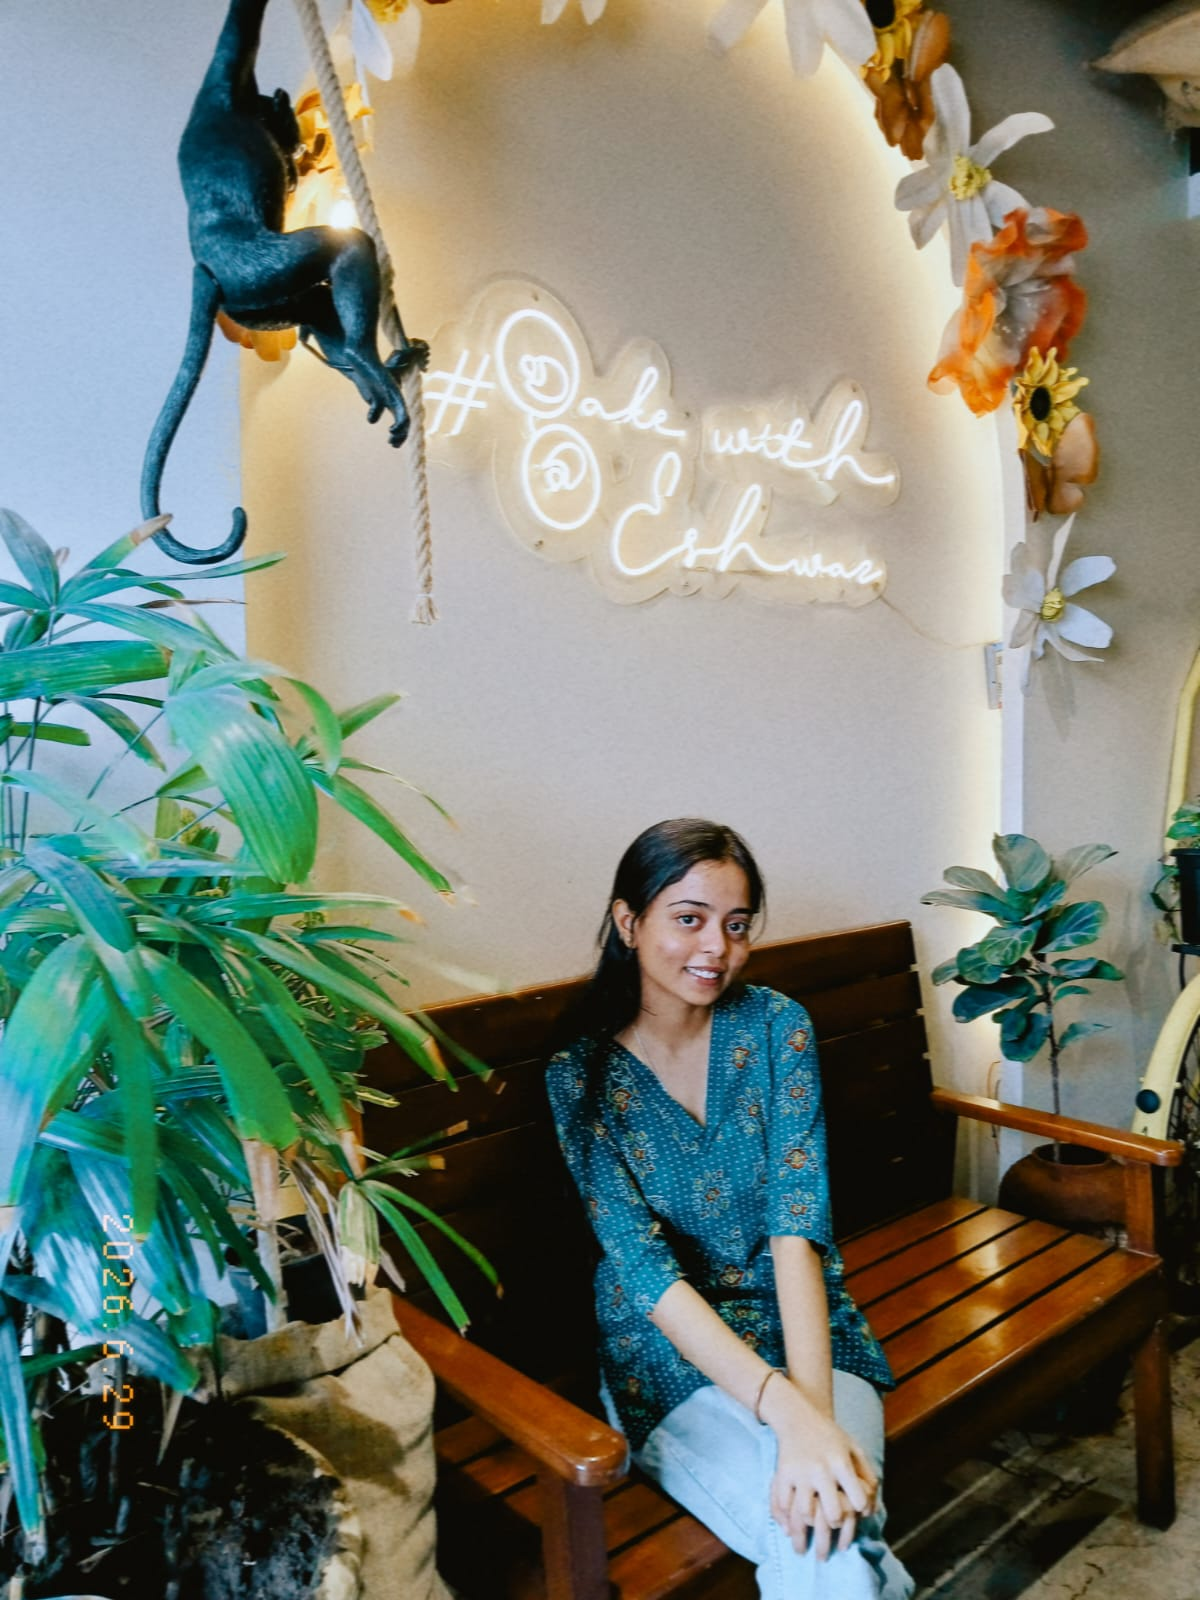
\includegraphics[width=0.55\textwidth]{image.jpeg}
  \caption{Reference input (\texttt{input/image.jpeg}), $1200\times1600$ portrait.}
  \label{fig:input}
\end{figure}

\begin{figure}[H]
  \centering
  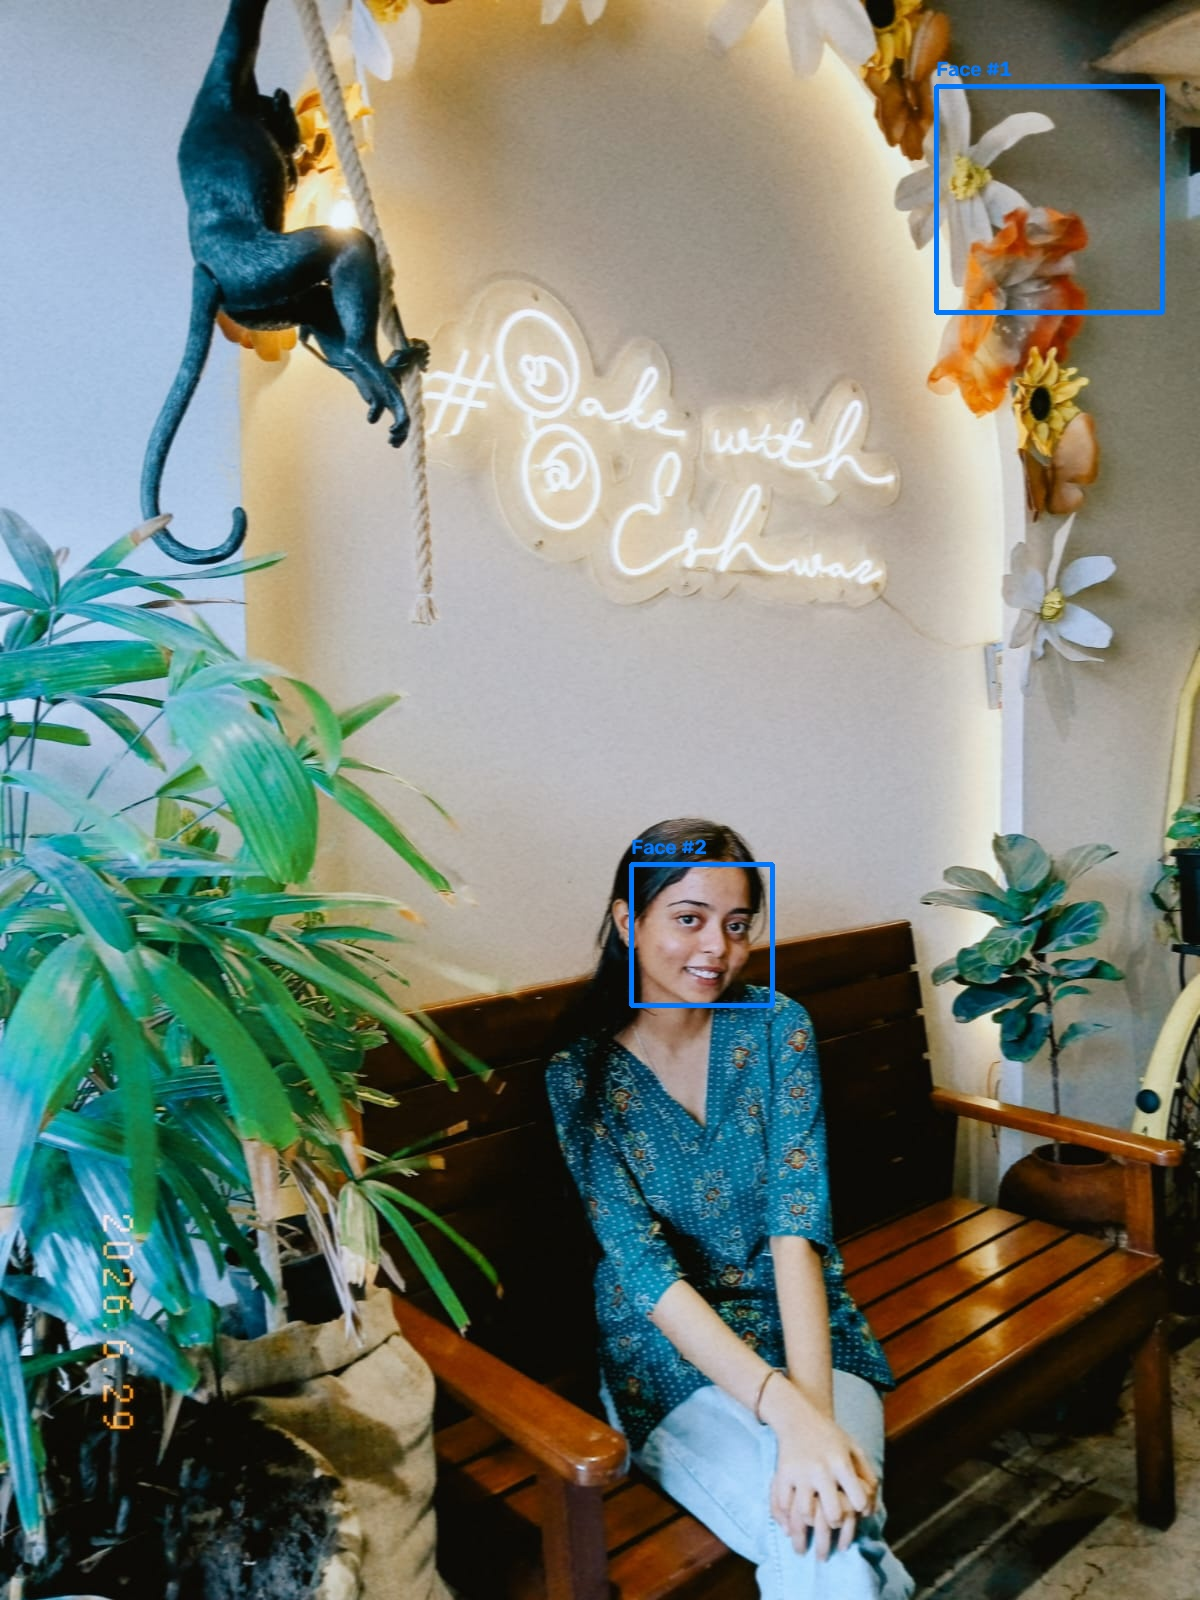
\includegraphics[width=0.55\textwidth]{annotated.jpg}
  \caption{Face marking: 2 numbered boxes on the reference photo.}
  \label{fig:marked}
\end{figure}

\begin{figure}[H]
  \centering
  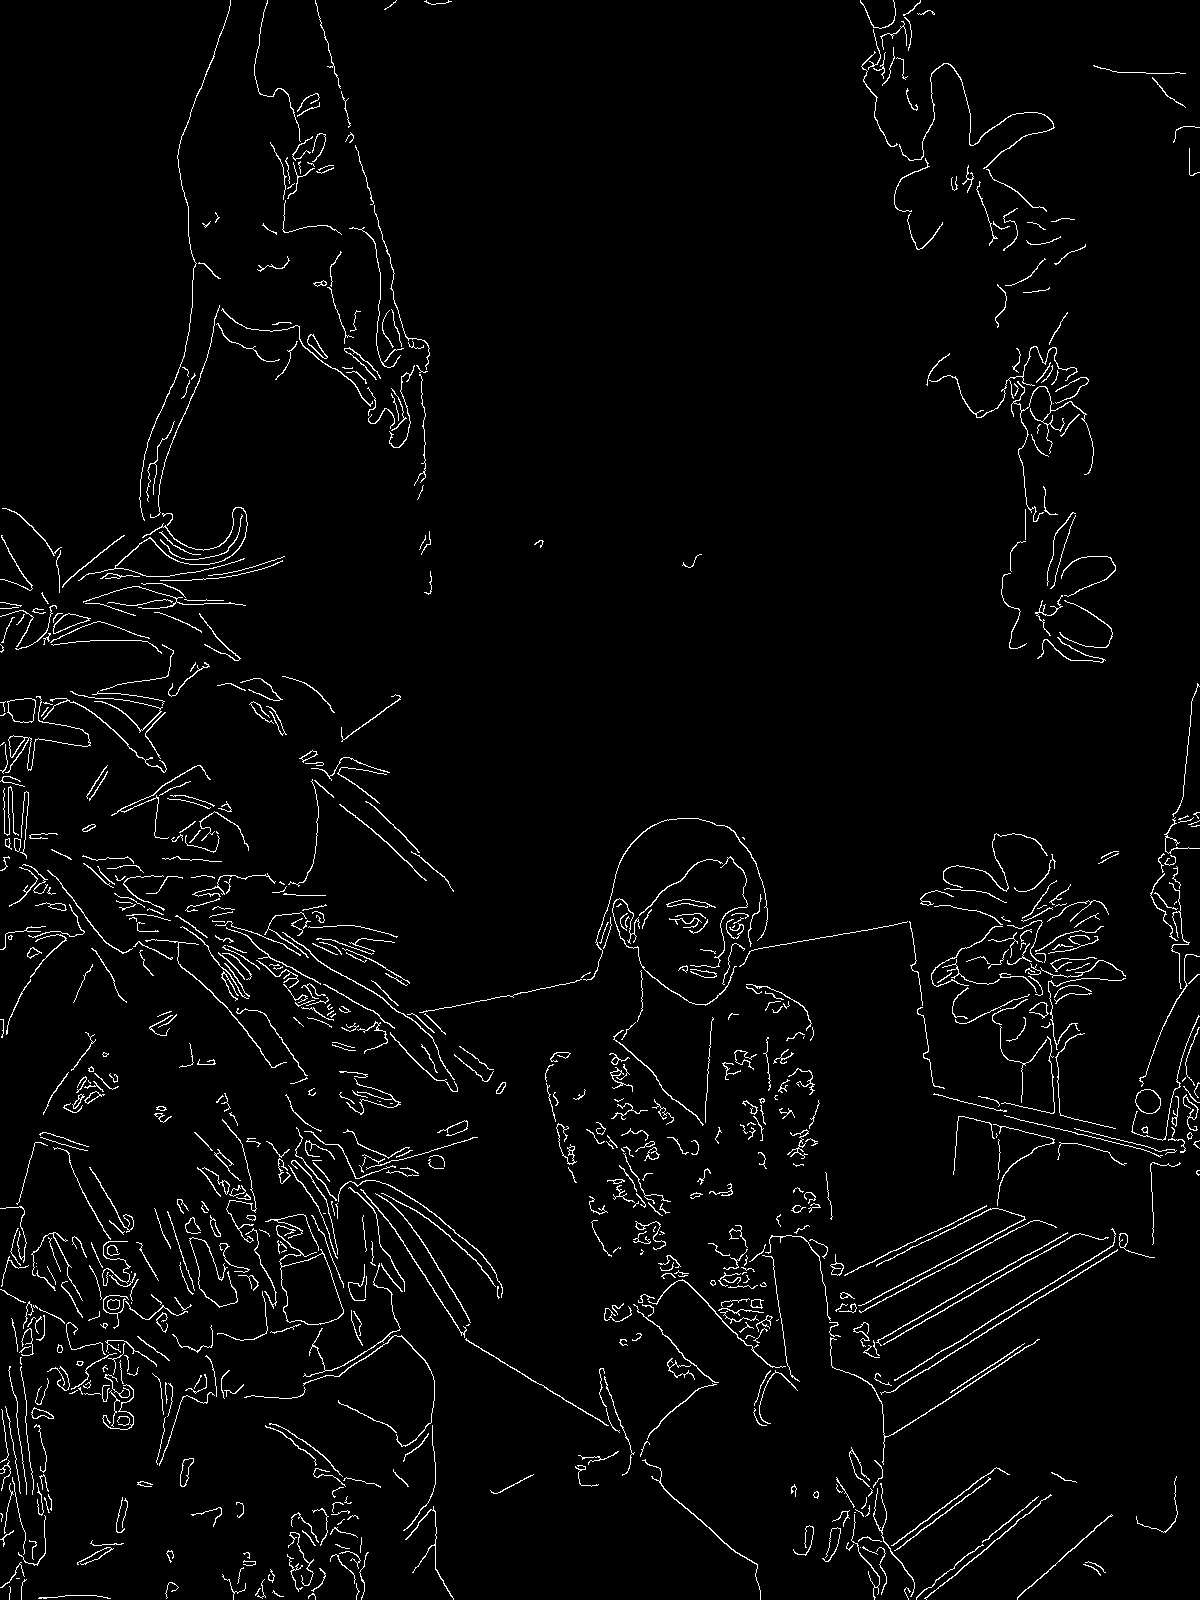
\includegraphics[width=0.55\textwidth]{edgemap.jpg}
  \caption{Structure map: Canny 60/140 after $7\times7$ blur (2.94\% active).}
  \label{fig:edges}
\end{figure}

\begin{lstlisting}[style=shell,caption={Console recap of the reference run}]
===== LensMetrics =====
Photo      : input/image.jpeg
Faces      : 2
Size       : 1200 x 1600 (portrait)
Exposure   : Well-exposed
Focus      : In-focus
Contours   : 859
Saved to   : output/ (annotated.jpg, edgemap.jpg, summary.txt, summary.json)
\end{lstlisting}

\begin{lstlisting}[style=shell,caption={Readable summary (output/summary.txt)}]
LensMetrics Inspection Summary
==============================

Source photo : input/image.jpeg
Faces marked : 2

[ Geometry ]
Resolution   : 1200 x 1600 (portrait)
Channels     : 3
Megapixels   : 1.92
Mean luma    : 123.8
Contrast     : 66.04

[ Clarity ]
Exposure     : Well-exposed (123.8)
Focus        : In-focus (score 122.02)

[ Structure ]
Edge pixels  : 56365 (2.94%)
Contours     : 859

[ Colour ]
B/G/R means  : 115.44 / 127.57 / 119.59
Dominant     : green
\end{lstlisting}

% ================= 12 =================
\section{Testing}
\subsection{Automated Suite}
Eight Pytest cases in \texttt{tests/test\_lensmetrics.py} use synthetic frames
(mid-grey, black, red-tinted) plus a temporary directory for report I/O:

\begin{lstlisting}[style=shell,caption={Full suite result}]
tests/test_lensmetrics.py::test_geometry_and_orientation PASSED      [ 12%]
tests/test_lensmetrics.py::test_clarity_mid_grey_is_well_exposed PASSED [ 25%]
tests/test_lensmetrics.py::test_dark_frame_flags_under_exposed PASSED [ 37%]
tests/test_lensmetrics.py::test_structure_map_shape_and_census PASSED [ 50%]
tests/test_lensmetrics.py::test_palette_reports_dominant_channel PASSED [ 62%]
tests/test_lensmetrics.py::test_face_tagging_keeps_dimensions PASSED [ 75%]
tests/test_lensmetrics.py::test_reports_write_txt_and_json PASSED    [ 87%]
tests/test_lensmetrics.py::test_bad_paths_raise_helpful_errors PASSED [100%]

8 passed in 0.20s
\end{lstlisting}

\subsection{Manual Checks}
\begin{center}
\footnotesize
\begin{tabularx}{\textwidth}{p{3.2cm}p{4.4cm}Xc}
\toprule
\textbf{Check} & \textbf{Expectation} & \textbf{Observation} & \textbf{Verdict} \\
\midrule
Reference photo & 4 artefacts written & annotated + edge map + txt + json present & PASS \\
Missing file & Path quoted in error & \texttt{No photo found at: \dots} & PASS \\
\texttt{.txt} as input & Suffix error + allowed list & Clear \texttt{ValueError} & PASS \\
Exposure label & Well-exposed at 123.8 & Matches band 55--195 & PASS \\
Focus label & In-focus at 122.02 & Above cutoff 90 & PASS \\
Edge density & Ratio in [0,1] & 0.0294 on reference & PASS \\
JSON schema & Tool + boxes + sections & All keys present & PASS \\
\bottomrule
\end{tabularx}
\end{center}

% ================= 13 =================
\section{Difficulties and Fixes}
\begin{enumerate}[leftmargin=1.5em]
  \item \textbf{Cascade file vanished in OpenCV 5.} \texttt{cv2.data.haarcascades}
    no longer ships the XML, so the first run failed to initialise.
    \textit{Fix:} vendor the cascade under \texttt{lensmetrics/models/} with a
    fallback to the install path --- reproducible on any wheel.
  \item \textbf{Cutoffs felt arbitrary.} Early brightness bands disagreed with
    test shots. \textit{Fix:} re-tuned to 55/195 for exposure and 90 for focus
    against dark, mid, and bright frames, and exposed them as CLI flags.
  \item \textbf{Even blur kernels crash Canny tuning.} An even kernel size
    silently misbehaves. \textit{Fix:} coerce even values up by one inside
    \texttt{trace\_structure}.
  \item \textbf{Text and JSON drifted.} Two writers meant two truths.
    \textit{Fix:} single \texttt{save\_reports} builds both from one payload.
\end{enumerate}

% ================= 14 =================
\section{Takeaways, Limits, and Next Steps}
\subsection{Takeaways}
Quantitative grades beat adjectives; dataclasses keep analysers honest and
testable; vendoring data files beats assuming install layouts; one payload
feeding two report formats prevents an entire class of bugs.

\subsection{Limits}
One photo per run; classical cascade misses profiled or occluded faces;
hard-wired defaults suit general shots, not night or document scans; no GUI.

\subsection{Next Steps}
Batch-folder mode with a CSV index; optional DNN face path when weights are
present; histogram PNGs beside the JSON; SSIM/noise metrics; a minimal
drag-and-drop front end.

% ================= 15 =================
\section{References}
\begin{enumerate}[leftmargin=1.5em]
  \item OpenCV team, \textit{OpenCV Documentation}, \url{https://docs.opencv.org/}.
  \item Viola, P. \& Jones, M., ``Rapid object detection using a boosted cascade
    of simple features,'' \emph{CVPR}, 2001.
  \item Canny, J., ``A computational approach to edge detection,''
    \emph{IEEE TPAMI}, 8(6), 1986.
  \item Bradski, G. \& Kaehler, A., \textit{Learning OpenCV}, O'Reilly, 2008.
  \item NumPy developers, \textit{NumPy Documentation}, \url{https://numpy.org/doc/stable/}.
  \item pytest developers, \textit{pytest Documentation}, \url{https://docs.pytest.org/}.
  \item Python Software Foundation, \textit{argparse Documentation},
    \url{https://docs.python.org/3/library/argparse.html}.
\end{enumerate}

% ================= 16 =================
\section{Closing}
LensMetrics turns an idle photo into a graded, illustrated record in under a
second on CPU: 2 faces boxed and logged, exposure and focus labelled from
measured cutoffs, 859 contours backing a 2.94\% edge-density figure, and a
colour profile naming green dominant --- with four artefacts and eight green
tests to prove it. The modular layout leaves clear seams for batch mode,
learned detectors, and richer metrics next.

\end{document}
